\documentclass[12pt]{extarticle}
%Some packages I commonly use.
\usepackage[portuguese]{babel}
\usepackage{graphicx}
\usepackage{framed}
\usepackage[normalem]{ulem}
\usepackage{amsmath}
\usepackage{amsthm}
\usepackage{amssymb}
\usepackage{amsfonts}
\usepackage{enumerate}
\usepackage[utf8]{inputenc}
\usepackage{float}
\usepackage{gensymb}
\usepackage[top=1 in,bottom=1in, left=1 in, right=1 in]{geometry}
\usepackage{multirow}
\usepackage{caption}
\usepackage{subcaption}
\usepackage[utf8]{inputenc}

%A bunch of definitions that make my life easier
\newcommand{\matlab}{{\sc Matlab} }
\newcommand{\cvec}[1]{{\mathbf #1}}
\newcommand{\rvec}[1]{\vec{\mathbf #1}}
\newcommand{\ihat}{\hat{\textbf{\i}}}
\newcommand{\jhat}{\hat{\textbf{\j}}}
\newcommand{\khat}{\hat{\textbf{k}}}
\newcommand{\minor}{{\rm minor}}
\newcommand{\trace}{{\rm trace}}
\newcommand{\spn}{{\rm Span}}
\newcommand{\rem}{{\rm rem}}
\newcommand{\ran}{{\rm range}}
\newcommand{\range}{{\rm range}}
\newcommand{\mdiv}{{\rm div}}
\newcommand{\proj}{{\rm proj}}
\newcommand{\R}{\mathbb{R}}
\newcommand{\N}{\mathbb{N}}
\newcommand{\Q}{\mathbb{Q}}
\newcommand{\Z}{\mathbb{Z}}
\newcommand{\<}{\langle}
\renewcommand{\>}{\rangle}
\renewcommand{\emptyset}{\varnothing}
\newcommand{\attn}[1]{\textbf{#1}}
\theoremstyle{definition}
\newtheorem{theorem}{Theorem}
\newtheorem{corollary}{Corollary}
\newtheorem*{definition}{Definition}
\newtheorem*{example}{Example}
\newtheorem*{note}{Note}
\newtheorem{exercise}{Exercise}
\newcommand{\bproof}{\bigskip {\bf Proof. }}
\newcommand{\eproof}{\hfill\qedsymbol}
\newcommand{\Disp}{\displaystyle}
\newcommand{\qe}{\hfill\(\bigtriangledown\)}
\setlength{\columnseprule}{1 pt}
\usepackage[utf8]{inputenc}

\title{Aula 5  - Propagação de Calor}
\author{Felipe Salvador}
\date{Atualizado em \today}

\begin{document}

\maketitle

\section{Introdução}
Nessa aula, quais são os mecanismos de transferência de um corpo para o outro e sob quais condições elas ocorrem com mais facilidade e como evitar a propagação de calor para outros corpos.

Ao todo, temos 3 processos de transferência de energia térmica ou propagação de calor: \textbf{condução, convecção e irradiação.} Vamos lembrar a regra de ouro para a propagação de calor: \textbf{Só acontece a transferência de calor quando há uma diferença de temperatura entre 2 corpos.}

\section{Condução}

\textbf{É o processo de transferência de calor por meio do contato físico entre corpos com temperaturas diferentes, por exemplo: encostar um corpo mais quente num corpo mais frio.}

Quando começo a aquecer a ponta de uma barra, ela começa a transferir calor para o resto da barra, aquecendo o resto da barra também. 
\begin{figure}[h]
    \centering
    \begin{subfigure}[b]{0.4\textwidth}
         \centering
         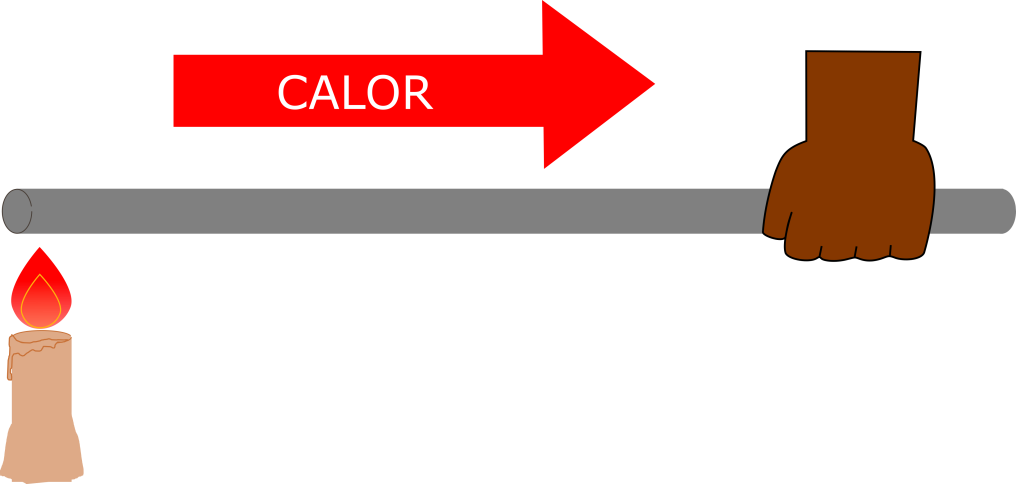
\includegraphics[width=\textwidth]{conducao.png}
         \caption{Condução de calor numa barra sendo aquecida numa ponta. Como a temperatura de uma ponta é maior que da outra ponta, há um fluxo de calor da ponta mais quente para a mais fria, aquecendo o resto da barra.}
         \label{fig:cond_1}
     \end{subfigure}
     \hfill
     \begin{subfigure}[b]{0.4\textwidth}
         \centering
         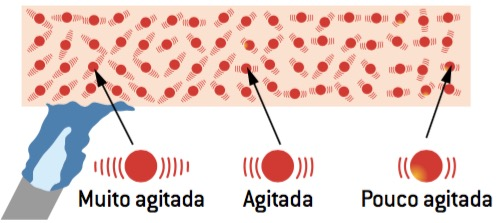
\includegraphics[width=\textwidth]{20190503-transmissao-calor.jpg}
         \caption{Ilustração da vibração das moléculas de uma barra sendo aquecida. A transferência de calor acontece quando as moléculas mais agitadas começam a dar um pouco de energia para as vizinhas menos agitadas.}
         \label{fig:cond_2}
     \end{subfigure}
\end{figure}

Importante ressaltar que se eu não parar de aquecer, a temperatura da barra não será homogênea, ou seja, cada parte da barra terá uma temperatura diferente. Esse processo todo depende do material que está sendo usado, além das dimensões do objeto.

Existe uma relação que quantifica o fluxo de calor por uma barra:
\begin{equation}
    \phi = K\frac{A\,(T_1 - T_2)}{d}
\end{equation}

\noindent em que '$\phi$' é o fluxo de calor, '$K$' é a condutibilidade térmica do material da barra, 'A' é a área da seção transversal da barra, $T_1,\,T_2$ são as temperaturas em cada ponta da barra e 'd' é o comprimento da barra.

'$K$' tem a dimensão de '$\frac{cal}{cm\,s\,^\circ C}$' e quanto maior for '$K$', mais calor é transmitido pela barra. \textbf{Portanto, materiais que conduzem bem o calor, tem '$K$' grande, enquanto materiais que conduzem mal o calor ou isolantes térmicos, possuem '$K$' bem pequeno.}

\section{Convecção}
\textbf{A convecção acontece somente nos fluídos (líquidos e gases) e é caracterizada pelo movimento de partes desses fluídos que estejam mais quente e também mais frios.}

A principal razão para que haja o movimento é que \textbf{partes dos fluídos com maior temperatura, ocupam mais espaço e tem menor densidade, enquanto partes mais frias são mais densas.}
Com isso, a parte do fluído mais densas caminha em direção ao fundo do volume, enquanto as partes menos densas vão para topo. 

Então, o fluxo de calor é feito pelo movimento das partículas com maior temperatura de um lugar para outro, como na figura a seguir:
\begin{figure}[h]
    \centering
    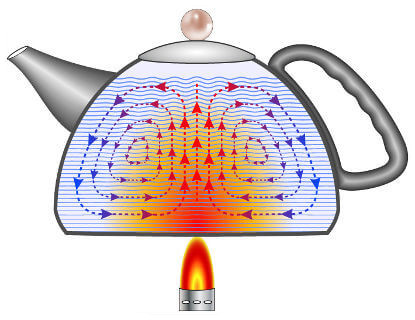
\includegraphics[width=0.6\textwidth]{conveccao-no-bule-5c2e5b51c413a.jpg}
    \caption{Ilustração da convecção. A água no fundo do bule é aquecida, logo a densidade diminui, fazendo essa parte da água subir. Ao chegar no topo, a temperatura da água diminui, porque o ar rouba um pouco de temperatura, aumentando a densidade da água, fazendo ela descer e o ciclo recomeça.}
    \label{fig:convecção}
\end{figure}

Esse é o princípio da geladeira. \textbf{O congelador fica em cima, porque é onde o ar frio entra, diminuindo ao máximo a temperatura dos alimentos. Conforme o ar vai descendo até o fundo da geladeira, ele vai ganhando a temperatura dos alimentos e, por contrapartida, resfriando-os. Assim, o congelador fica bem mais frio do que a geladeira.}
    
    Outra questão importante é a altura de um ar-condicionado. Colocamos o ar-condicionado no alto da parede, porque o ar frio irá descer e forçar o ar quente subir, assim esfriando esse ar quente, que torna-se frio e o ciclo recomeça.
    
    Quando colocamos o ar-condicionado perto do chão, o ar quente sobe, enquanto o ar frio fica perto do chão, mas o ar quente não é resfriado, assim o quarto não fica gelado.
    
    A mesma explicação é o porquê de uma lareira estar perto do chão.

\section{Irradiação}

\textbf{É o processo de transmissão de calor por meios de ondas (eletromagnéticas). Esse é o processo que não precisa de um contato físico para transmitir calor.} Basta ter um corpo com uma temperatura maior que o ambiente que ele está para que ele comece a irradiar calor para o ambiente.

Esse é o processo que o Sol transmite luz e calor para a Terra. O porquê da Terra não ser totalmente fria a noite, é a existência de uma atmosfera que faz o papel de uma 'cúpula' que não permite que essas ondas de calor da irradiação vá para o espaço. Dessa forma, todo o calor fica na Terra, mantendo ela aquecida. \textbf{Esse fenômeno é chamado de Efeito Estufa}, pois a atmosfera funciona como uma estufa.
\begin{figure}[h]
    \centering
    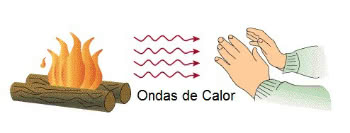
\includegraphics[width=0.6\textwidth]{ir_1.jpg}
    \caption{Ilustração da irradiação de calor. As ondas de calor irradiadas pela fogueira aquece a nossa mão.}
    \label{fig:irradiacao}
\end{figure}

Porém, nem todo corpo absorve as ondas da irradiação. Os corpos podem ser classificados de 3 formas:
\begin{itemize}
    \item \textbf{Opacos} - é quando um corpo absorve nada do calor que as ondas da irradiação transmitem;
    \item \textbf{Transparentes} - é quando o corpo absorve parcialmente o calor transmitido pelas ondas;
    \item \textbf{Negro} - é quando o corpo absorve todo o calor transmitido pelas ondas da irradiação.
\end{itemize}

Um exemplo de um objeto que evita os 3 processos de transmissão de calor (condução, convecção e irradiação) é a \textbf{Garrafa Térmica}:

\begin{figure}[h]
    \centering
    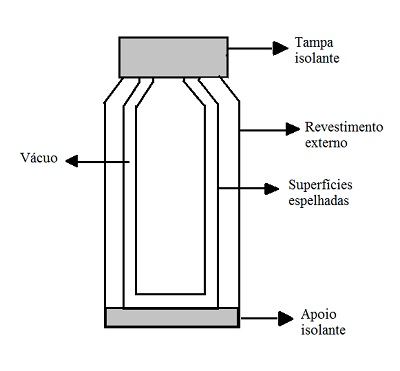
\includegraphics[width=0.6\textwidth]{composição de uma garrafa térmica.jpg}
    \caption{Diagrama de uma garrafa térmica - ela é composta por 2 paredes internas com vácuo entre elas, assim a condução térmica não acontece; a parede interna é revestida por um material espelhado, assim a irradiação não acontece dentro da garrafa; e a tampa de rosca, é para evitar a convecção, assim o líquido não perde temperatura por estar em contato com o ambiente, evitando a convecção.}
    \label{fig:my_label}
\end{figure}
\end{document}
